\section{Schema Evaluation}
\label{sec:schema_eval}
Our first study evaluated the quality of individual schema formulas learned by NESL. We presented learned schema formulas from the \texttt{:Steps} and \texttt{:Goals} sections to human annotators and asked them to rate the quality of the formula, given the schema topic, on a 1-5 Likert scale. The prompt given to the evaluators was the following:
\begin{displayquote}
\textit{The statement above is a reasonably clear, entirely plausible general claim and seems neither too specific nor too general or vague to be useful.}
\end{displayquote}
This prompt is due to \citet{knext-eval}, who used it to elicit evaluations of quality of automatically acquired knowledge formulas from the \textsc{KNEXT} acquisition system. It incorporates three key dimensions into one quality rating: \textbf{clarity} of the representation, and \textbf{plausibility} and \textbf{generality} of the claim.

\subsection{Dataset}
Evaluators rated steps and goals from 43 schemas generated by NESL. The 43 topics used to generate the schemas were manually selected by a research assistant from a list of topics produced by a prompt-engineered, GPT-J 6B-based story summarization program executed on a set of 300 ROCstories; the research assistant selected topics they deemed to be sensible. Latent schema sampling was performed with a story sample count of eight for each learned schema. The following topics were used for schema generation in the schema quality evaluation experiment:

\scalebox{0.75}{
\vbox{
\begin{multicols}{3}
\begin{itemize}
\footnotesize
\item \texttt{being at a concert}
\item \texttt{being at the beach}
\item \texttt{being scared}
\item \texttt{calling the radio}
\item \texttt{cleaning your house}
\item \texttt{cooking}
\item \texttt{feeding a baby}
\item \texttt{finding a lost pet}
\item \texttt{getting into an accident}
\item \texttt{getting mail}
\item \texttt{going fishing}
\item \texttt{going to the library}
\item \texttt{going to the store}
\item \texttt{growing plants}
\item \texttt{having a cabin}
\item \texttt{having a friend over}
\item \texttt{having a meal}
\item \texttt{hiking}
\item \texttt{holding a concert}
\item \texttt{learning an instrument}
\item \texttt{looking for a place to eat}
\item \texttt{mailing a letter}
\item \texttt{making friends}
\item \texttt{meeting someone}
\item \texttt{milking a cow}
\item \texttt{moving to a new place}
\item \texttt{packing for a trip}
\item \texttt{playing baseball}
\item \texttt{playing in the snow}
\item \texttt{playing outside}
\item \texttt{playing with a ball}
\item \texttt{playing with a pet}
\item \texttt{rainy weather}
\item \texttt{school}
\item \texttt{seeing a movie}
\item \texttt{shopping}
\item \texttt{showering}
\item \texttt{taking care of an animal}
\item \texttt{throwing things away}
\item \texttt{vacationing}
\item \texttt{visiting a farm}
\item \texttt{walking through the woods}
\item \texttt{washing clothes}
\end{itemize}
\end{multicols}
}
}

\subsection{Comparisons}
\label{sec:comparison}
Prior work on human evaluation of automatically acquired script-like knowledge has used comparable evaluation strategies, although human evaluation of acquired script-like knowledge lacks a standard study design. Here, we discuss several similar projects with whose human evaluation results we juxtapose our own, as well as differences between their study designs and ours to be aware of when comparing the scores.

\citet{pichotta2016learning}, whose inferred event tuples were rated on a Likert scale, with values ranging from \textit{Very Unlikely} to \textit{Very Likely}, by human evaluators. While the semantics of the prompt are more ambiguous than our \textsc{KNEXT}-derived prompt, the normalized results are comparable. \citet{weber_causal_scripts} evaluate acquired knowledge using two metrics, one of which is the \textit{event chain completion} metric, in which human evaluators rate the likelihood of a predicted event given a chain of preceding events. The comparison of this metric to ours is arguably the least direct, as we evaluate the likelihood of an event predicated on the truth of the schema's \textit{topic}; however, under the assumption that the given events in the event chain completion metric sufficiently characterize an implicit schema topic to the human evaluator, a comparison is possible. \citet{goal-oriented-scripts} ask human evaluators to \textit{edit} learned scripts by either re-ordering their steps or deleting irrelevant steps. This leads to an approximation of schema relevance defined by the ratio of edited script length to original script length, i.e. how many of the learned events were judged to be irrelevant. \citet{starsem-scripts} manually evaluate their own script events for topical relevance, among other things.

The most common human evaluation metric in this compared prior work is \textit{relevance} to the schema topic. Our evaluation prompt jointly asked for evaluation of plausibility given the schema topic, clarity, and balance of generality/specificity, of which only the first dimension -- plausibility -- is comparable to other relevance evaluations. While we believe all of these dimensions are still important, the confounded formulation of the KNEXT prompt led us to split evaluations in the inference evaluation study presented in Section~\ref{sec:inf_eval} into three dimensions.

\subsection{Results}
We present the results of the ungrounded schema evaluation study in Table~\ref{tab:schema_results}, along with the results of the similar studies discussed in Section~\ref{sec:comparison}. We present results for step and goal formulas separately to illustrate the significant difference in average score. Another notable score differential is the one between NESL formulas when presented to annotators as tabreps vs. GPT-verbalized sentences: the average score in the latter case is significantly higher.

\begin{table}[ht]
    \centering
    \begin{tabular}{l|l|l}
       \textbf{System} & \textbf{Average Step Score} & \textbf{Average Goal Score} \\
       \hline
       \citet{pichotta2016learning} & 0.662 & --- \\
              %\hline
       \citet{weber_causal_scripts} & 0.601 & --- \\
              %\hline
       \citet{goal-oriented-scripts} \textsc{(generative)} & 0.390 & --- \\
              %\hline
       \citet{goal-oriented-scripts} \textsc{(SIO)} & 0.700 & --- \\
              %\hline
       \citet{starsem-scripts} & 0.771 & --- \\
              %\hline
              %\hline
       \textsc{NESL (tabrep)} & 0.615 & 0.518 \\
              %\hline
       \textsc{NESL (GPT)} & 0.735 & 0.524 \\
    \end{tabular}
    \caption{Average quality scores for steps of learned schemas/scripts across several learning systems. Scores have been normalized to a 0-1 range.}
    \label{tab:schema_results}
\end{table}

\begin{figure}
\centering
\begin{minipage}[t][.4\textheight]{.38\columnwidth}
    \centering
    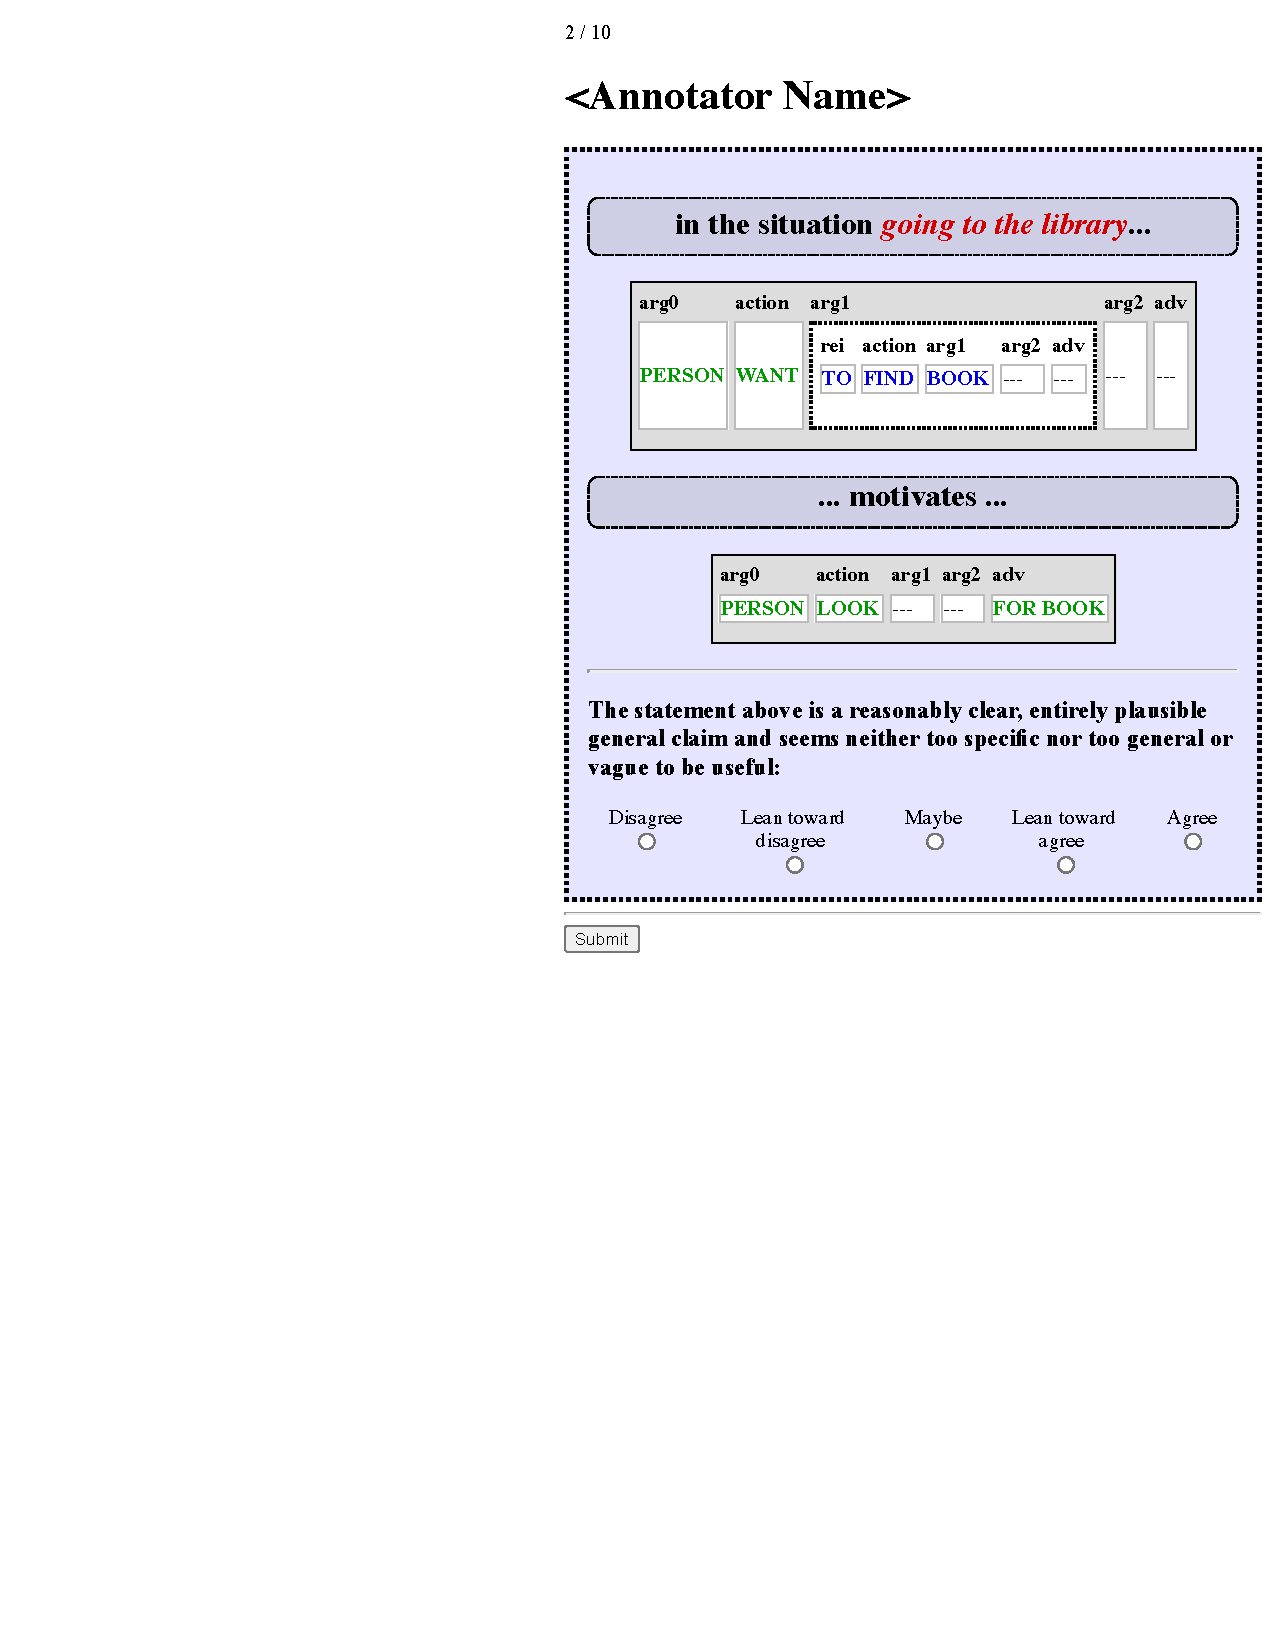
\includegraphics[width=\textwidth]{CH4_learning/evaleg4.pdf}
    \caption{An example of a form presented to a schema quality evaluator for a \textit{goal} formula.}
    \label{fig:goal_eval_eg}
\end{minipage}%
\hfill
\begin{minipage}[t][.4\textheight]{.4\columnwidth}
    \centering
    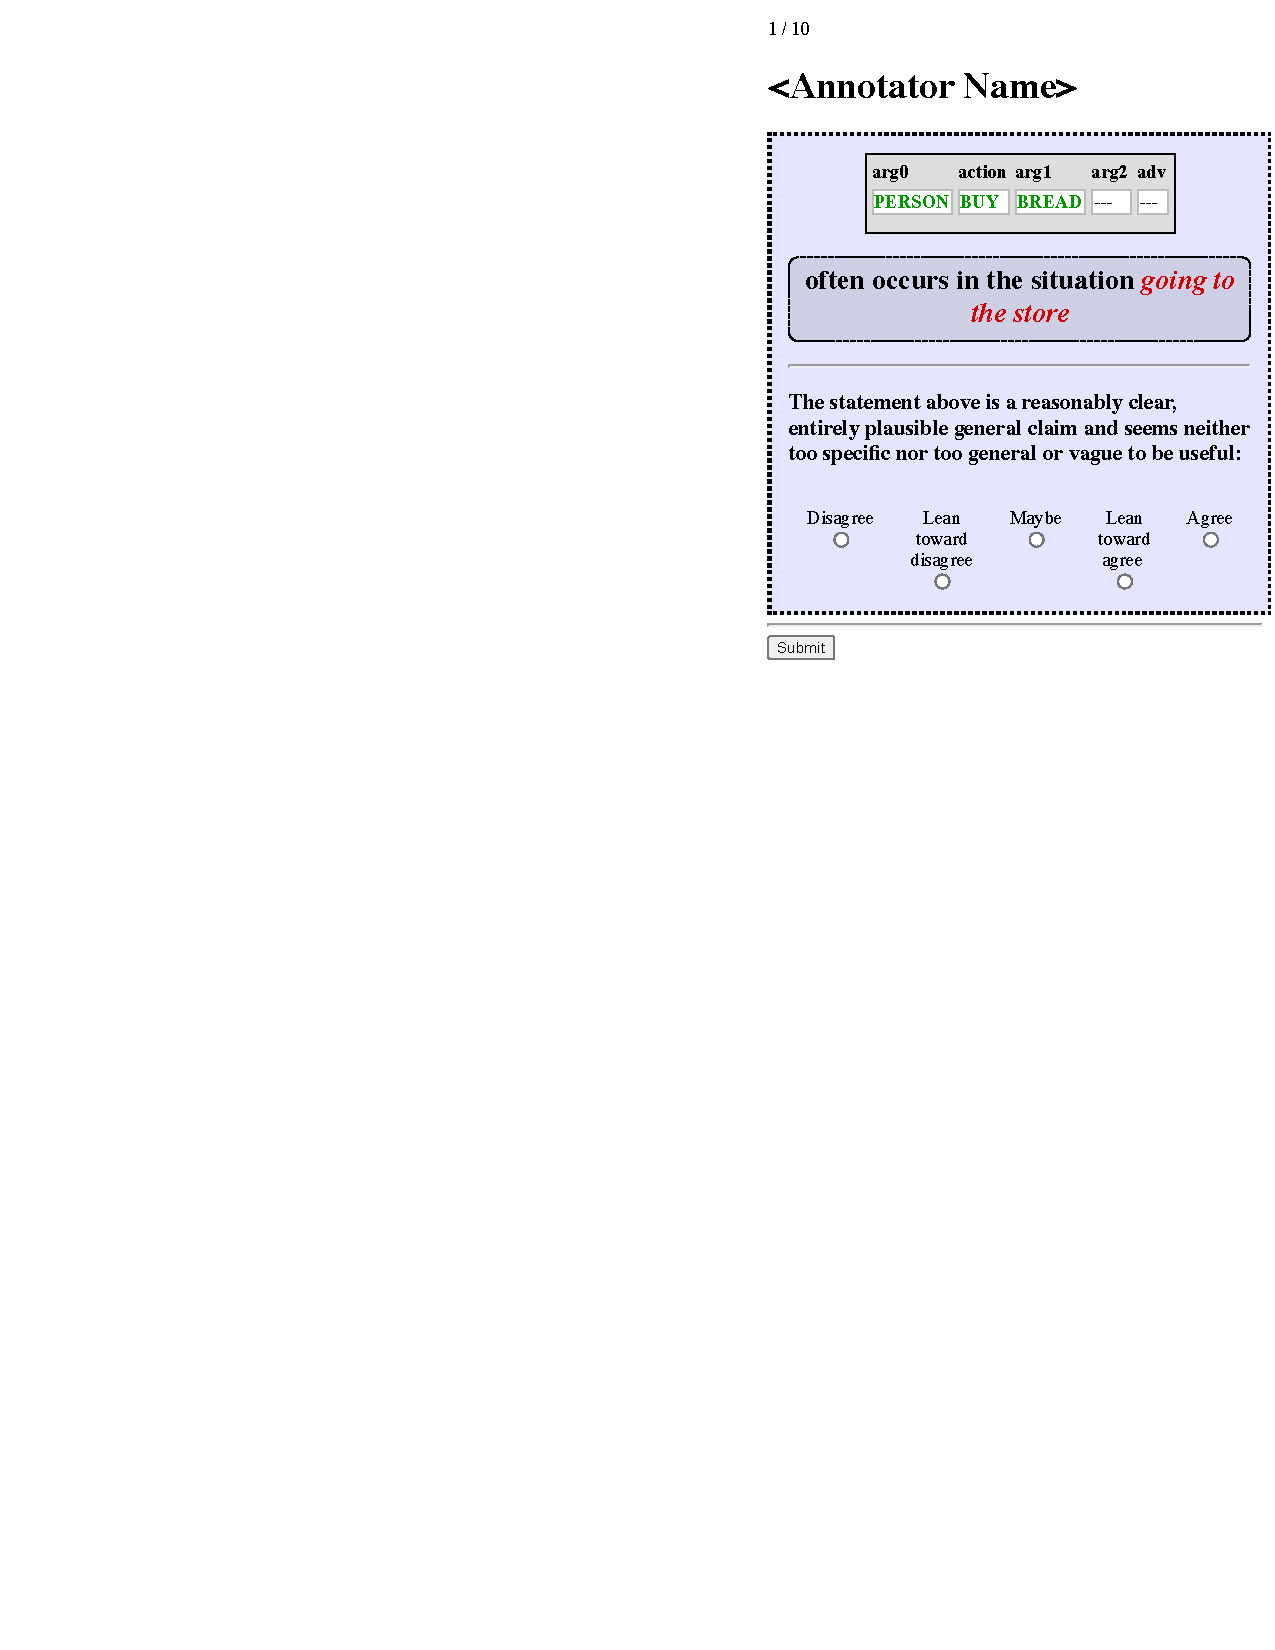
\includegraphics[width=\textwidth]{CH4_learning/evaleg3.pdf}
    \caption{An example of a form presented to a schema quality evaluator for a \textit{step} formula.}
    \label{fig:step_eval_eg}
\end{minipage}
%\vfill
\begin{minipage}[b][.5\textheight]{0.8\columnwidth}
    \centering
    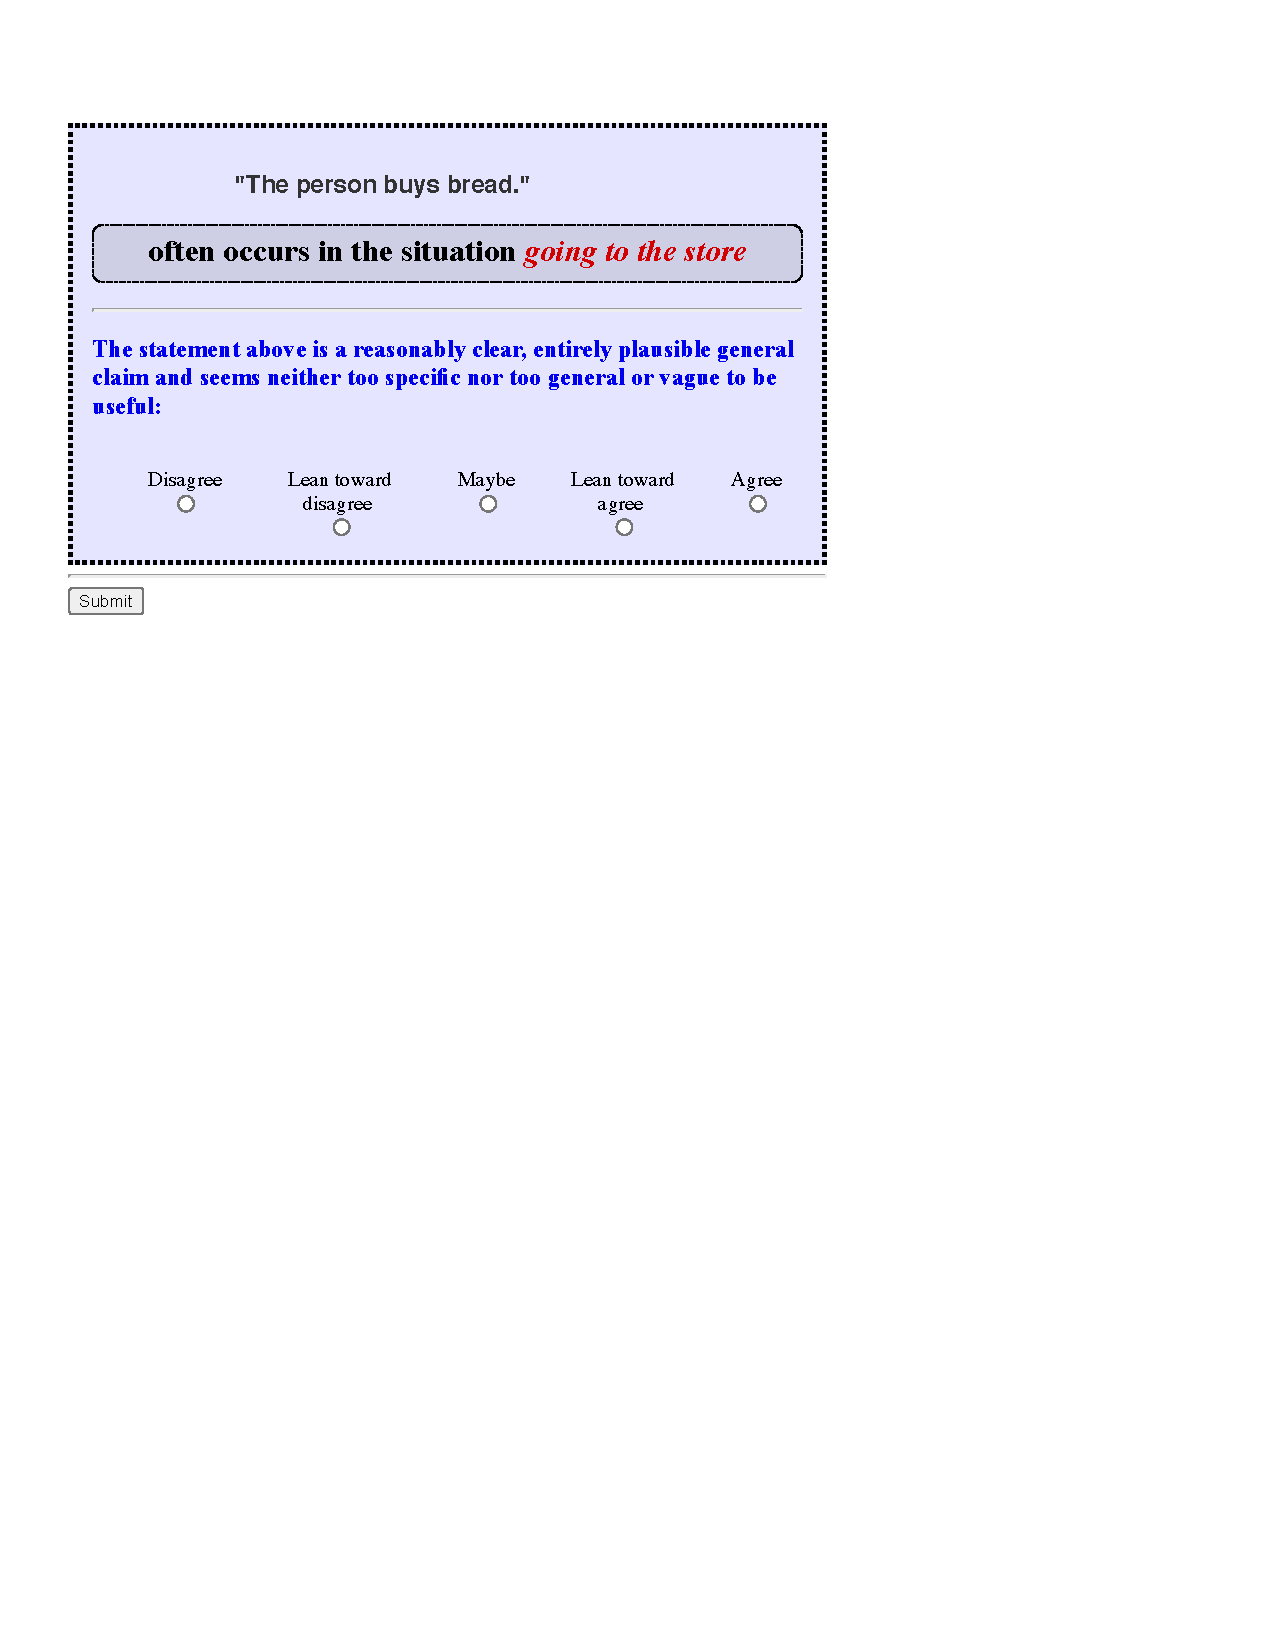
\includegraphics[width=0.5\textwidth]{CH5_eval/gpteval}
    \caption{An example of a form presented to a schema quality evaluator for a \textit{step} formula that has been rendered, using GPT-2, into natural English. This corresponds to the \textit{tabular} version shown in Figure~\ref{fig:step_eval_eg}.}
    \label{fig:gpt_step_eval_eg}
\end{minipage}

\end{figure}


\begin{figure}
    \centering

\end{figure}